\documentclass[runningheads]{llncs}
%
\usepackage[T1]{fontenc}
\usepackage{tikz}
\usetikzlibrary{arrows.meta, positioning, calc, backgrounds, fit, shadows.blur}
\usetikzlibrary{shadows}
% T1 fonts will be used to generate the final print and online PDFs,
% so please use T1 fonts in your manuscript whenever possible.
% Other font encodings may result in incorrect characters.
%
% Hyperref package for clickable links
\usepackage{hyperref}
%
\usepackage{graphicx}
% Used for displaying a sample figure. If possible, figure files should
% be included in EPS format.
%
% If you use the hyperref package, please uncomment the following two lines
% to display URLs in blue roman font according to Springer's eBook style:
\usepackage{color}
\renewcommand\UrlFont{\color{blue}\rmfamily}
\urlstyle{rm}
\usepackage{amsmath}
\usepackage{amssymb}
\usepackage{tikz}
\usetikzlibrary{positioning,arrows.meta,fit,backgrounds}
%\usepackage{algorithm}
%\usepackage{algpseudocode}
\usepackage[ruled,vlined]{algorithm2e}
\usepackage{fixme}
\fxsetup{draft}


\allowdisplaybreaks

\newcommand{\rGB}{\textsc{$r$-GB} }
\newcommand{\rGBP}{$r$-GBP }

\makeatletter
\AtBeginDocument{%
	\renewcommand\doi[1]{}%
}
\makeatother

% cSpell:enable

\begin{document}
	
 
\section{Workflow visualization}
  
 \begin{figure}[!ht]
 	\raggedright
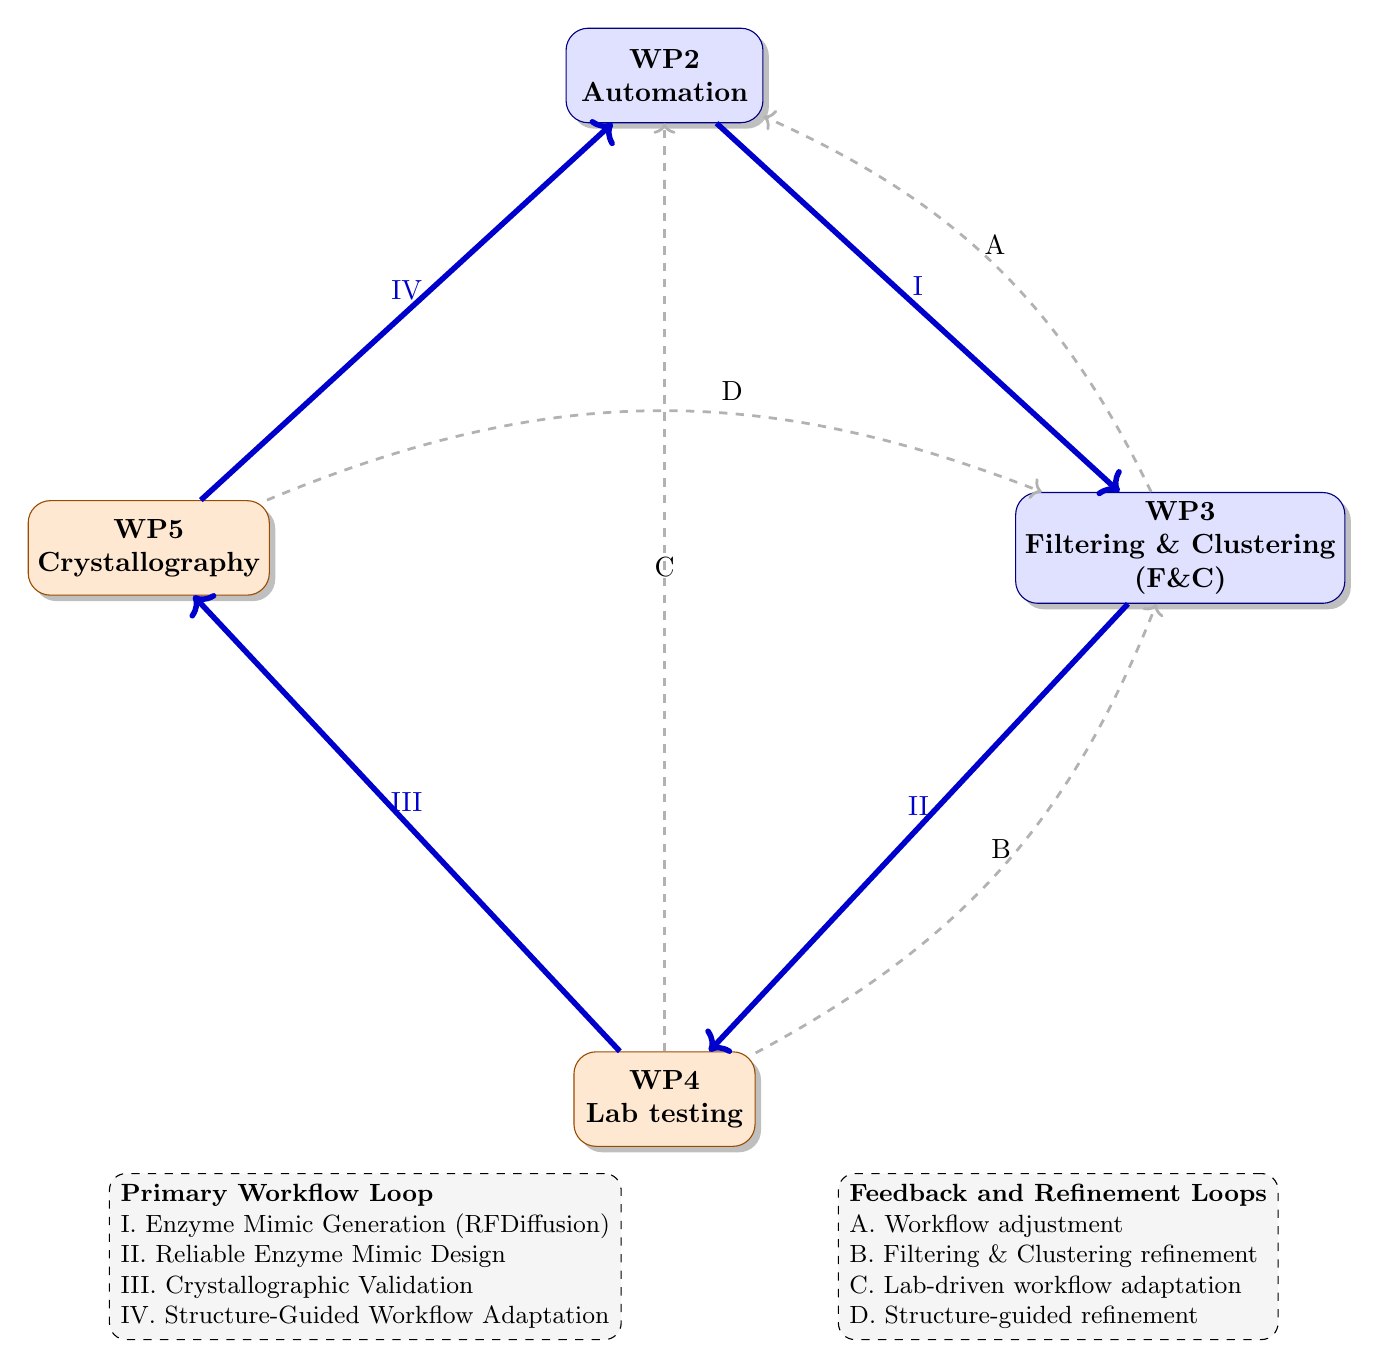
\begin{tikzpicture}[xshift=-2.5cm, 
	every node/.style={draw, rectangle, rounded corners, minimum width=1.0cm, minimum height=0.3cm, align=center},
    mainarrow/.style={->, line width=2pt, color=blue!80!black},
    feedback/.style={->, dashed, line width=1pt,    color=gray!60},
	lab/.style={
		draw,
		dashed,
		rounded corners=6pt,
		fill=gray!8,
		font=\small,
		align=center,
		inner sep=4pt
	},
	wp/.style={
		draw,
		rectangle,
		rounded corners=8pt,
		minimum width=2.5cm,
		minimum height=1.2cm,
		align=center,
		font=\bfseries,
		fill=blue!12,
		draw=blue!50!black,
		drop shadow
	},
	wp_exp/.style={
		draw,
		rectangle,
		rounded corners=8pt,
		minimum width=2.3cm,
		minimum height=1.2cm,
		align=center,
		font=\bfseries,
		fill=orange!18,
		draw=orange!60!black,
		drop shadow
	}
	]
	
	% Nodes in circular layout
	\node[wp] (WP2) at (90:6cm) {WP2\\Automation};
	\node[wp] (WP3) at (0:6.55cm) {WP3\\Filtering \& Clustering \\ (F\&C)};
	\node[wp_exp] (WP4) at (-90:7cm) {WP4 \\ Lab testing};
	\node[wp_exp] (WP5) at (180:6.55cm) {WP5\\Crystallography};
	
    \draw[mainarrow] (WP2) to[bend left=0] node[midway, above, draw=none]{I}(WP3);
    \draw[mainarrow] (WP3) to[bend left=0] node[midway, above, draw=none]{II} (WP4);
    \draw[mainarrow] (WP4) to[bend left=0] node[midway, above, draw=none]{III} (WP5);
    \draw[mainarrow] (WP5) to[bend left=0] node[midway, above, draw=none]{IV} (WP2);
	
	% Feedback arrows (clean, no labels)
	\draw[feedback] (WP3) to[bend right=20] node[midway, above, draw=none, fill=none, text=black]{A} (WP2);
	\draw[feedback] (WP4) to[bend right=20] node[midway, above, draw=none, fill=none, text=black]{B} (WP3);
	\draw[feedback] (WP4) to[bend right=0] node[midway, above, draw=none, fill=none, text=black]{C} (WP2);
	\draw[feedback] (WP5) to[bend right=-22] node[midway, above, draw=none, fill=none, xshift=1cm, text=black]{D} (WP3);
 
	
	
	% External annotations (clean placement)
	%\node[lab, align=left] at (-3.0, 0.8) 
	%{
	%	Filtering \& Clustering \\
	%	refinement
	%};
	%{- Crystallography \\ \ \ active site conformation\\
	% - Substrate binding};
	 
	%\node[lab, align=left] at (-3.0,-4.2) 
	%{  
	%	Christallography validation
	%};
	%{  - E. coli expression \\
	%   - protein characterization\\
	%   - activity assay};
		
	%\node[lab, align=left] at (-3.0, 3.0) 
    %{ Crystallography-based \\ workflow      
    %  adaption
    %};
	
	%\node[lab, align=left] at (0.0, -3.0) 
	%{  
	%	Data-based workflow \\
	%	adoption
	%};

	%\node[lab, align=left] at (6.0, -3.0) 
   %{  
   %  	Filtering \& Clustering \\
   %	    adjustment
   %};
   
 % \node[lab, align=left] at (5.8, 3.0) 
 % {  
 %	 Filtering \& Clustering-based \\
 %	  workflow adaption
 %};

\node[lab, align=left] at (-3.8, -9.0)
{ \textbf{Primary Workflow Loop} \\
	I. Enzyme Mimic Generation (RFDiffusion) \\
	II. Reliable Enzyme Mimic Design \\
	III. Crystallographic Validation \\
	IV. Structure-Guided Workflow Adaptation
};

\node[lab, align=left] at (5.0, -9.0)
{ \textbf{Feedback and Refinement Loops} \\
	A. Workflow adjustment \\
	B. Filtering \& Clustering refinement \\
	C. Lab-driven workflow adaptation \\
	D. Structure-guided refinement };

\end{tikzpicture}

  \end{figure}
 

\textit{Explanations}.  
WP2 automation consists of several steps, roughly speaking we have:
\begin{itemize}
	\item Enzyme structure generation based on the use of \texttt{RFDiffusion} 
	\item Deep Learning utilization (\texttt{ProteinMPNN}) to predict sequences that suite realistically  to these structures (multiple of them)
	\item The generated sequence serve as input of \texttt{AlphaFokd} which generate a set of structures for these sequences.
\end{itemize}
 
 In order to balance intensification and diversification of the search towards generation of Enzyme mimics (EMs) with a preserved catalytic functionality of the reference enzyme, two complementary techniques are  employed: \textbf{filtering} and \textbf{clustering} techniques. 
 
 
 \textit{Filtering techniques} utilize different scores to measure structural distance between generated enzymes (their structures) from the reference enzyme and filter out those based on biologically-motivated threshold value. One of the used measure is the well-known the rooted mean square deviation (RMSD). In this way, we try to narrow the search towards those with potentially more functional enzymes with an inherited catalytic property. \\
 
 \textit{Clustering techniques} serve to diversify the search, thus spread the search uniformly in the space of EMs. In order to be able to utilize the classical clustering such as k-means or agglomerative clustering, we map the search of EMs into the structural space. As EMs are represented as graphs (with a threshold value), examples of the graphs of several EMs from our preliminary experimental analysis are given in Figures~\ref{fig:1}--\ref{fig:2}.
 
 \begin{figure}[!ht]
 	 \centering
     \includegraphics[width=200pt,height=100pt]{enzyme\_mimicB1-501-379-00EN379a\_B1-501-379-00-enzyme\_mimicB1-501-379-00EN379a-ranked\_0.png}
     \caption{\texttt{enzyme\_mimicB1-501-379-00EN379a\_B1-501-379-00-enzyme\_mimicB1-501-379-00EN379a-ranked\_0.png}}
     \label{fig:1}
     
 \end{figure}
 
 
  
 \begin{figure}[!ht]
 	\centering
 	\includegraphics[width=200pt,height=100pt]{enzyme\_mimicB1-501-379-03EN379i\_B1-501-379-03-enzyme\_mimicB1-501-379-03EN379i-ranked\_0.png}
 	\caption{\texttt{enzyme\_mimicB1-501-379-03EN379i\_B1-501-379-03-enzyme\_mimicB1-501-379-03EN379i-ranked\_0.png}}
 	\label{fig:2}
 	
 \end{figure}
 
 
\subsection{Protein Structure Graph Construction and Feature Extraction}

To enable graph-based analysis of enzyme structures, each Protein Data Bank (PDB) file is transformed into an undirected residue interaction graph using Bio.PDB from \texttt{BioPython} library. Let $G=(V,E)$ denote the resulting graph, where vertices represent amino acid residues and edges represent spatial proximity relationships between residues.

\paragraph{Graph Construction.}
For each protein structure, only residues containing a C$_\alpha$ atom are considered. Each residue is represented as a vertex
\[
v_i \in V,
\]
where $v_i$ corresponds to the $i$-th amino acid residue in the protein chain. The Cartesian coordinates of the residue are taken from its C$_\alpha$ atom.

Two vertices $v_i$ and $v_j$ are connected by an undirected edge if the Euclidean distance between their C$_\alpha$ atoms is below a predefined threshold $\tau$:
\[
(v_i,v_j)\in E
\quad \Longleftrightarrow \quad
\|\mathbf{x}_i-\mathbf{x}_j\|_2 \leq \tau ,
\]
where $\mathbf{x}_i$ and $\mathbf{x}_j$ denote the coordinates of the corresponding C$_\alpha$ atoms. In our implementation, we use
\[
\tau = 8 \, \text{\AA}.
\]

This representation captures the spatial organization of the protein and encodes residue-residue contacts as graph edges.

\paragraph{Extracted Graph Features.}
For each graph, a set of topological descriptors is computed to characterize its structural properties.

\begin{itemize}
	\item \textbf{Number of nodes}
	\[
	n = |V|,
	\]
	corresponding to the total number of amino acid residues.
	
	\item \textbf{Number of edges}
	\[
	m = |E|,
	\]
	representing the number of residue-residue contacts.
	
	\item \textbf{Graph density}
	\[
	D = \frac{2m}{n(n-1)},
	\]
	measuring how densely connected the graph is.
	
	\item \textbf{Average degree}
	\[
	\bar{k} = \frac{2m}{n},
	\]
	indicating the average number of neighboring residues.
	
	\item \textbf{Minimum and maximum degree}
	\[
	k_{\min} = \min_{v \in V} \deg(v),
	\qquad
	k_{\max} = \max_{v \in V} \deg(v),
	\]
	describing the least and most connected residues.
	
	\item \textbf{Average clustering coefficient}
	\[
	C = \frac{1}{n}\sum_{v\in V} C(v),
	\]
	where $C(v)$ denotes the local clustering coefficient of vertex $v$. This metric quantifies the tendency of neighboring residues to form local clusters.
	
	\item \textbf{Number of connected components}
	\[
	c(G),
	\]
	representing the number of disconnected subgraphs.
	
	\item \textbf{Degree centrality}
	For each residue,
	\[
	DC(v)=\frac{\deg(v)}{n-1}.
	\]
	From these values, both the average and maximum degree centrality are recorded:
	\[
	\overline{DC}
	=
	\frac{1}{n}
	\sum_{v\in V}DC(v),
	\]
	\[
	DC_{\max}
	=
	\max_{v\in V}DC(v).
	\]
	
	\item \textbf{Diameter}
	If the graph is connected, the diameter is computed as
	\[
	\mathrm{diam}(G)
	=
	\max_{u,v\in V} d(u,v),
	\]
	where $d(u,v)$ is the shortest-path distance between vertices $u$ and $v$.
	
	\item \textbf{Average shortest-path length}
	For connected graphs,
	\[
	L
	=
	\frac{1}{n(n-1)}
	\sum_{u\neq v} d(u,v),
	\]
	measuring the average number of graph hops required to connect two residues.
\end{itemize}

These graph descriptors provide a compact representation of the protein's structural organization and can subsequently be used as input features for filtering, clustering, and machine-learning models aimed at identifying structurally diverse yet functionally plausible enzyme candidates.

\begin{figure}[!ht]
	\centering
     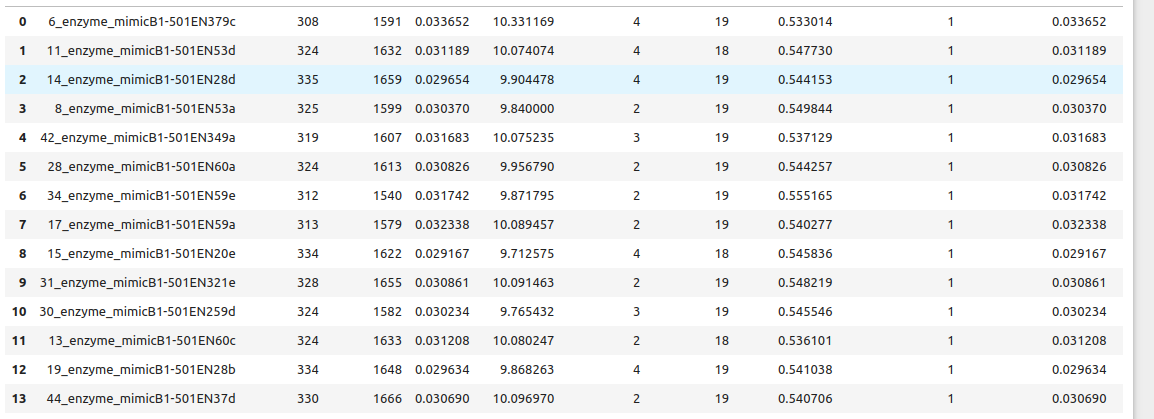
\includegraphics[width=350pt,height=200pt]{structure_feature_space.png}
     \caption{DataFrame of enzyme structures and their features}
\end{figure}
 
 Clustering. Based on the best structures of each sequences generated from \texttt{AlphaFold} (50 structures), we have applied a $k$-means algorithm, with a maximum $k$ value satisfying $silhouette \geq 0.25$ meaning to establish a reasonable set of clusters. 
 
 
 \begin{figure}[!ht]
 	\centering
 	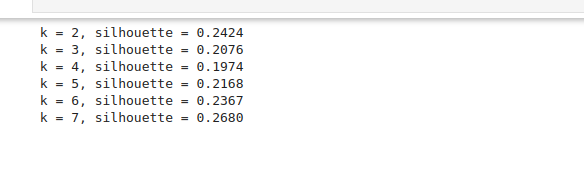
\includegraphics[width=350pt,height=100pt]{k_vals.png}
 	\caption{Different $k$ values obtained after applying k-means; somewhat suitable value selected is  $k=7$.}
 \end{figure}
 
 
  \begin{figure}[!ht]
 	\centering
 	\includegraphics[width=350pt,height=200pt]{cluster\_2dPCA.png}
 	\caption{2D PCA for the best clustering of the space of EMs obtained from the workflow.}
 \end{figure}
 
 \end{document}
